% This is samplepaper.tex, a sample chapter demonstrating the
% LLNCS macro package for Springer Computer Science proceedings;
% Version 2.20 of 2017/10/04
%
\documentclass[runningheads]{llncs}
%
\usepackage{graphicx}
\usepackage{float}
\usepackage{subcaption}
\usepackage{dirtytalk}
\captionsetup{compatibility=false}



% Used for displaying a sample figure. If possible, figure files should
% be included in EPS format.
%
% If you use the hyperref package, please uncomment the following line
% to display URLs in blue roman font according to Springer's eBook style:
% \renewcommand\UrlFont{\color{blue}\rmfamily}

\begin{document}
%
\title{Bachelor Dissertation}
%
%\titlerunning{Abbreviated paper title}
% If the paper title is too long for the running head, you can set
% an abbreviated paper title here
%
\author{Kasper Engelen\and
		Jonathan Meyer\and
		Dawid Miroyan\and
		Igor Schittekat}
%
%
\institute{University of Antwerp}
%
\maketitle              % typeset the header of the contribution
%
\begin{abstract}
This document reports our findings regarding the final dissertation. The sections and subsections correspond to the assignments given to us. In this project we worked with a simulator called Stride, developed at the University of Antwerp. We explore various concepts within computational epidemiology through the use of this program. 

\keywords{Computational Epidemiology  \and Dissertation}
\end{abstract}
%
%
%
\section{Simulation}
\subsection{Stochastic Variation}

\paragraph{} The first topic we consider is stochastic variation. Since the simulation uses a pseudo-random number generator, it's useful to inspect the influence of this stochasticity on the results of the simulation. Using the Stan tool which is provided with Stride, we collected data on 100 simulations with an identical configuration file. The only difference between executions is the RNG seed. For the data we collected, we calculated a  mean of 33.33 new cases per day, and a variance of 1196.99. Looking at the plot for the cumulative cases per day, two 'categories' can be distinguished:  'outbreak' scenarios and 'extinction' scenarios. These cases are quite evenly spread, which explains the high variance for new cases per day. In the former, the curve has a sigmoid shape, indicating that the disease succesfully spread among the population. The latter scenario corresponds to the curves that are almost constant and are bounded by a value well under the population size. In these cases, the disease did not manage to spread, resulting in only a few infected people at the end of the simulation. This is likely explained by the initial infectation: if the first person to be infected is sufficiently isolated (either socially or by being surrounded by people who are immune), the disease doesn't have a chance to spread. From the boxplot and a normal probability plot for the average new cases per day (Figure \ref{normalPlots}) (without extincion cases), it seems like the new cases per day do not have a normal distribution. However, the plot for new cases per day is very jagged (it jumps significantly from day to day), therefore this might not be representative. 
\\
Figure \ref{casesPlots} shows the different scenarios. In the cumulative cases plot the 'extinction' senario is clearly visible at the bottom. The plot for new cases per day is very jagged, which can also be explained by the stochastic nature of the simulation.

\begin{figure}[h!]
	\centering
	\begin{subfigure}[b]{0.7\linewidth}
		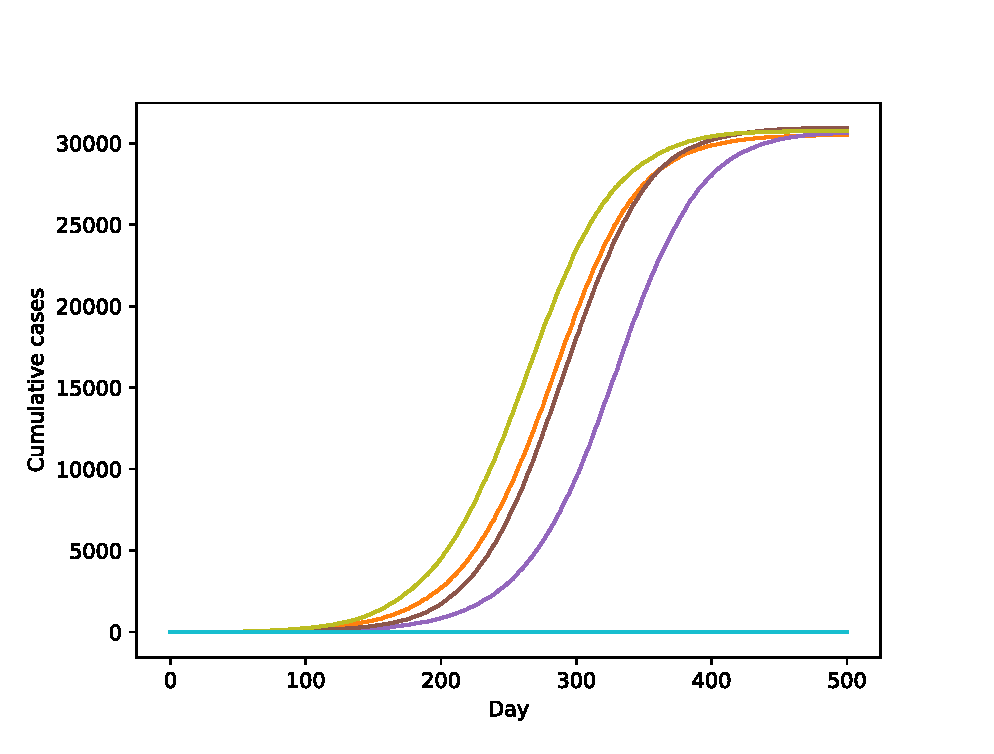
\includegraphics[width=\linewidth]{cases_cum.eps}
		\caption{Cumulative cases per day.}
	\end{subfigure}
	\begin{subfigure}[b]{0.7\linewidth}
		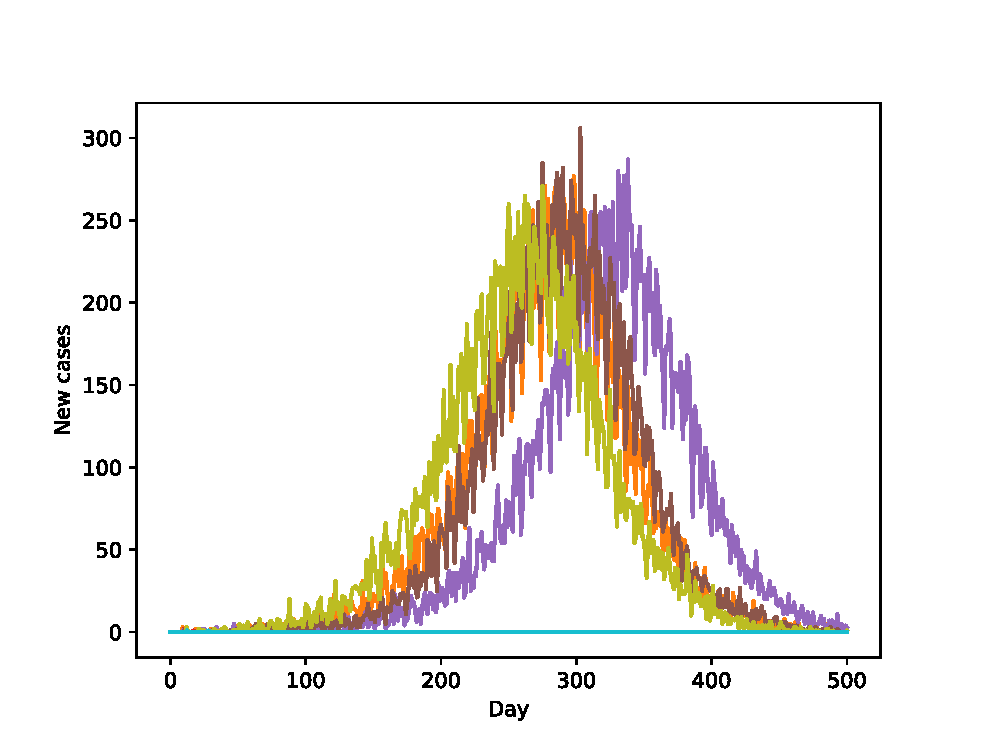
\includegraphics[width=\linewidth]{cases_per_day.eps}
		\caption{New cases per day.}
	\end{subfigure}
	\caption{Results of five different simulations, using a disease profile for measles. Seeding rate = $0.2$\%, $R_0$ = 11. Simulated for a population of 600,000, with 80\% vaccine and immunity rate.}
	\label{casesPlots}
\end{figure}
\clearpage

\begin{figure}[h!]
	\centering
	\begin{subfigure}[b]{0.7\linewidth}
		\includegraphics[width=\linewidth]{Boxplot.eps}
		\caption{Boxplot for average new cases per day.}
	\end{subfigure}
	\begin{subfigure}[b]{0.7\linewidth}
		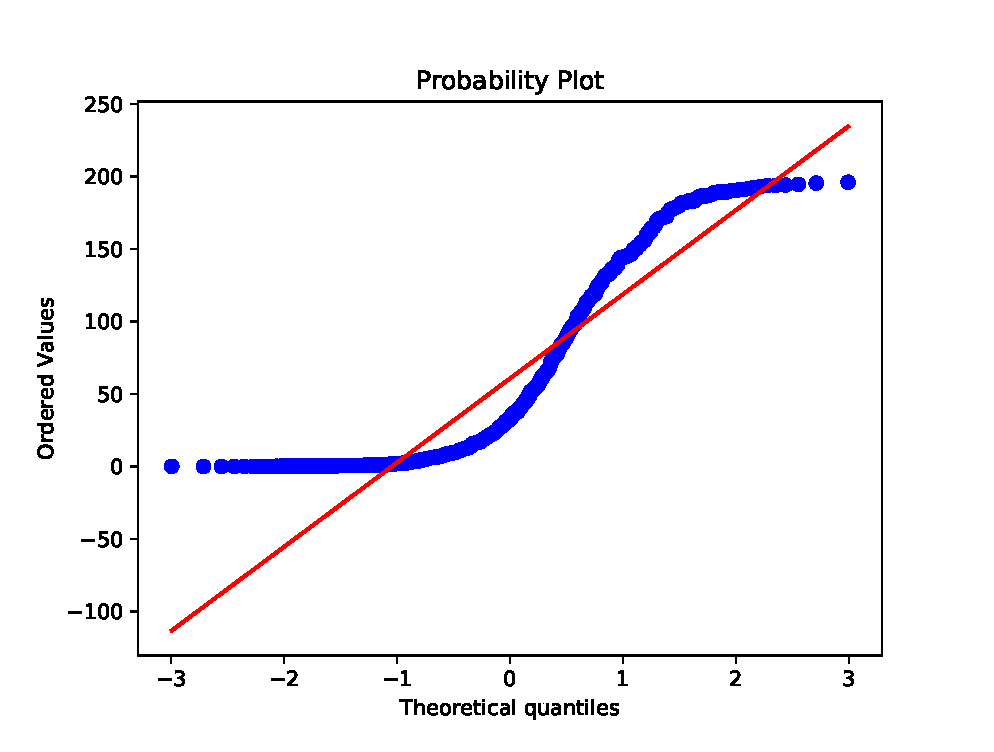
\includegraphics[width=\linewidth]{NormalDistProb.eps}
		\caption{Normal Distribution Plot for average new cases per day.}
	\end{subfigure}
	\caption{Results of 100 different simulations, using a disease profile for measles. Seeding rate = $0.2$\%, $R_0$ = 11. Simulated for a population of 600,000, with 80\% vaccine and immunity rate.}
	\label{normalPlots}
\end{figure}


\subsection{Extinction Threshold}

\paragraph{} As discussed previously, it might be the case that only very few people become infected over the course of a simulation. This is referred to as extinction. There is a clear distinction between outbreaks and extinctions, so in this subsection we attempt to find an \emph{extinction threshold}.

\paragraph{} Figure \ref{ETHist} gives the frequencies of the amount of infected people at the end of the simulations. The distinction between outbreaks and extinctions is quite clear from this histogram. There is one peak on the lower end of the x-axis, and there is a cluster on the higher-end. It is hard to find a good concrete value for the threshold, but the total amount of infected people in an extinction is always significantly under the total population size. Therefore, a fraction of the total population could be used as treshold. In our simulations the amount of cases after extinction never exceeded 50, so a threshold of 0.01\% of the population seems reasonable.

\begin{figure}[!h]
	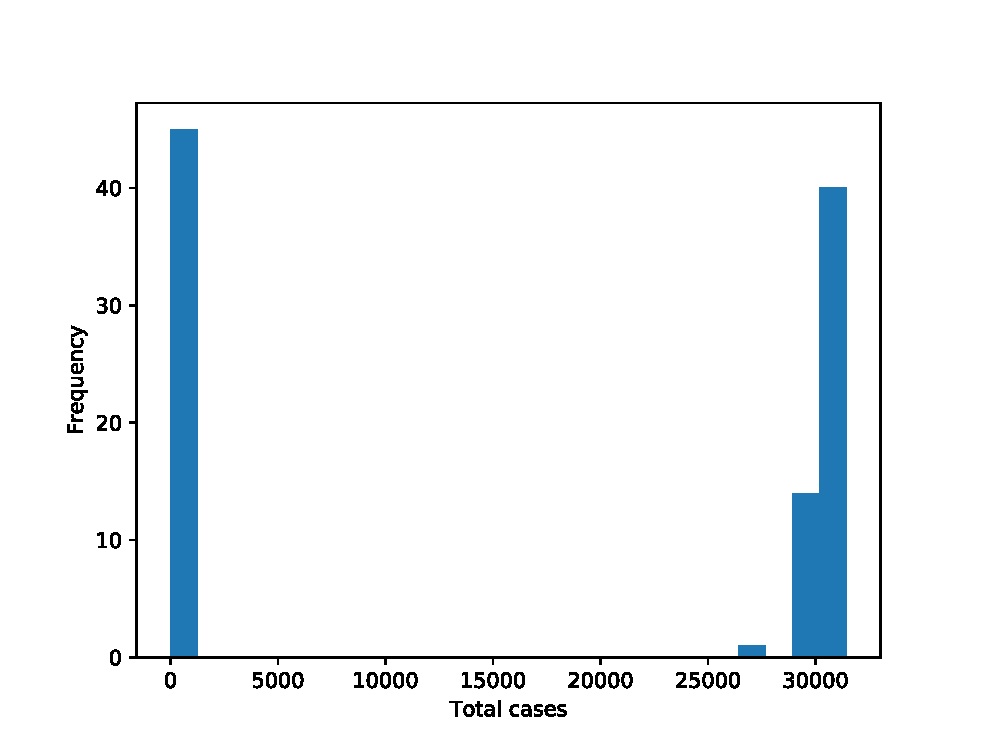
\includegraphics[width=\textwidth]{Hist.eps}
	\caption{Frequencies of final amounts of cases for 100 simulations, using a disease profile for measles. Seeding rate = $0.2$\%, $R_0$ = 11. Simulated for a population of 600,000, with 80\% vaccine and immunity rate.} 
	\label{ETHist}
\end{figure}

\subsection{Immunity Level}

\paragraph{} In order to make assumptions about the population's immunity level, we look at the simulated results for different values. Upon experimentation, it becomes apparent the immunity level is approximately 70\% of the population. Figure \ref{immLvlPlot} shows the average new cases per day for different immunity levels. The reference curve is also included. This plot was generated by taking the average of new cases per day over 20 simulations per immunity level. Using PyStride to simulate outbreaks, we narrowed down the immunity level $I$ to \( 0.705 \leq I \leq 0.7175 \).

\begin{figure}[H]
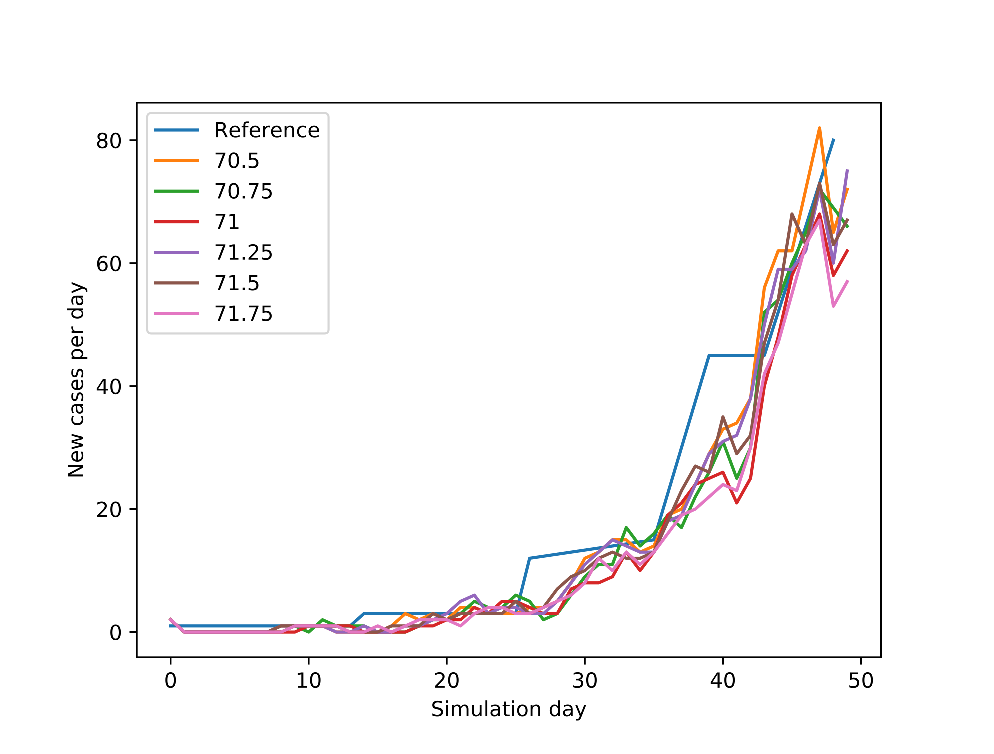
\includegraphics[width=\textwidth]{ImmLvl.eps}
\caption{Average new cases per day, calculated from 20 simulations per immunity level. Simulated using a disease profile for measles. Seeding rate = $0.000334$\%, $R_0$ = 15. Population size is 600,000, with random vaccine profile.} 
\label{immLvlPlot}
\end{figure}


\subsection{Estimating $R_{0}$}

\paragraph{} Now that we have a relatively decent estimate for the immunity level of the population, we can do an analogous exercise to estimate $R_0$. For this data, we fixed the immunity level to 70.5\%. Figure \ref{R0EstPlot} (a) shows the plot for each possible $R_0$ in the range $[12, 18]$ (average over 20 simulations). It's clear that the best candidates are 14, 15 or potentially 16. When we plot a more detailed plot for just those valued (average over 30 different simulations), it seems 15 is the best estimate for $R_0$.

\begin{figure}[H]
	\centering
	\begin{subfigure}[b]{0.7\linewidth}
		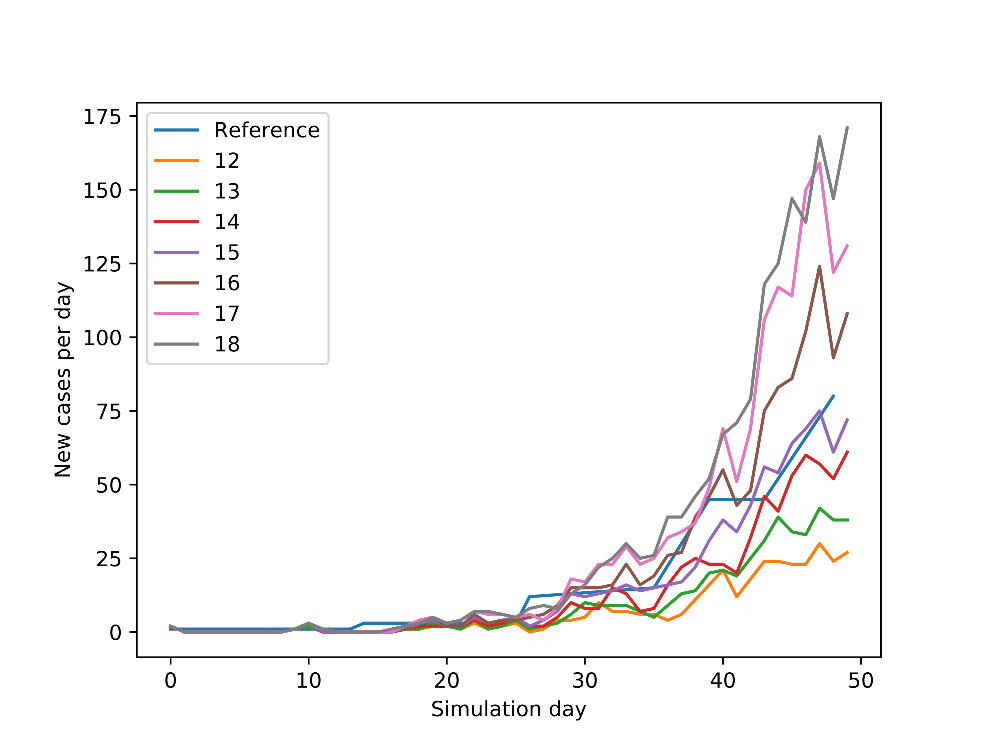
\includegraphics[width=\textwidth]{R0_all_20runs.eps}
		\caption{Overview of all potential $R_0$'s. Averages from 20 runs per $R_0$.} 	
	\end{subfigure}
	\begin{subfigure}[b]{0.7\linewidth}
		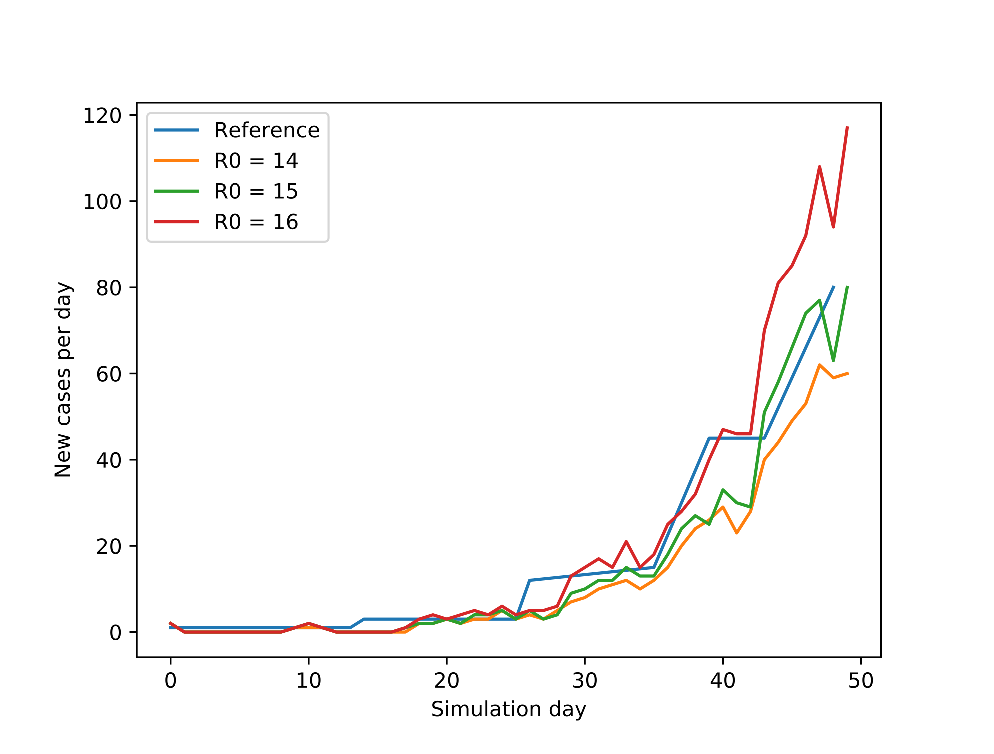
\includegraphics[width=\textwidth]{R0_detail_30runs.eps}
		\caption{More detailed look at $R_0$ candidates. Averages from 30 runs per $R_0$.} 
	\end{subfigure}
	\caption{Averages for different values of $R_0$.}
	\label{R0EstPlot}
\end{figure}

\section{Population generation}

In this section we will investigate what impact the population structure and generation has on the simulations. More specifically we will investigate the impact of the age distribution, the effectiveness of the vaccination of college students, and whether or not commuting to work has an effect on disease spread.

\subsection{Influence of demography}

% outbreak risico, outbreak grootte
\paragraph{} We want to determine whether or not the age distribution of a population has an impact on the size and probability of an outbreak. We start off with two populations, region A and region B, each generated based on a household file. The households mainly differ in age, with the households of region A being generally younger that those of region B. This is shown in figure \ref{2_1_regionDiff_plotAgeDistr}.

\begin{figure}[H]
\centering
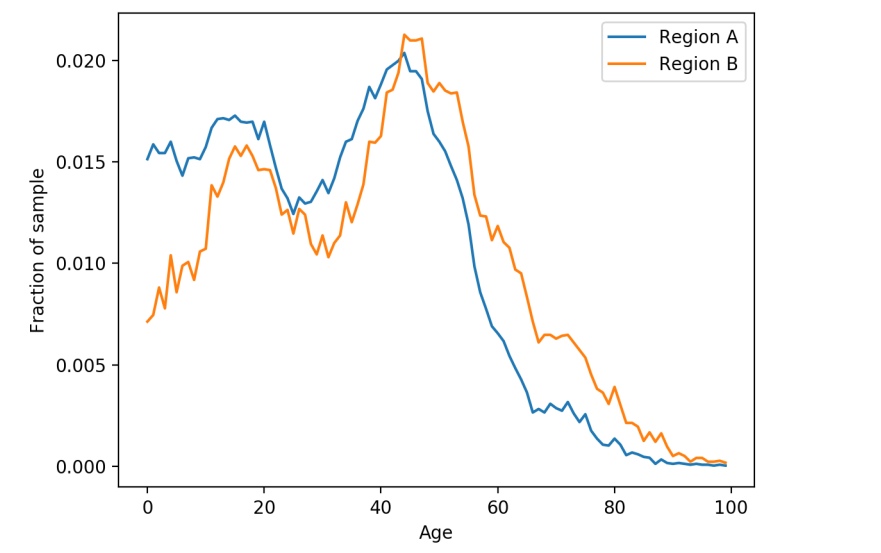
\includegraphics[width=0.8\textwidth]{./2_1_regionDiff/plot_ageDistr.png}
\caption{The age distribution of region A and region B.}
\label{2_1_regionDiff_plotAgeDistr}
\end{figure}

\paragraph{} In order to see the impact of the difference in age distribution on the simulation, we had to run a number of simulations. Each simulation we would run had to be \say{interesting}, i.e. when compared to other simulations the impact of the age difference had to be clear. We listed a number of parameter sets so that all regions, big and small seeding rates, short and long simulation lengths, and the difference in weekdays would be covered.

\begin{table}[H]
\centering
\begin{tabular}{|l|l|l|l|}
\hline
\textbf{Region} & \textbf{Seeding rate} & \textbf{Number of days} & \textbf{Weekday} \\
\hline
Region A & 0.002 &      50 Days & Monday \\ 
 \hline
Region A & 0.002 &      300 Days & Monday \\ 
 \hline
Region A & 0.0003 &     50 Days &  Monday \\ 
 \hline
Region A & 0.0003 &     300 Days & Monday \\ 
 \hline
Region A & 0.00000167 & 50 Days &  Monday \\ 
 \hline
Region A & 0.00000167 & 300 Days & Monday \\ 
 \hline
Region B & 0.002 &      50 Days &  Monday \\ 
 \hline
Region B & 0.002 &      300 Days & Monday \\ 
 \hline
Region B & 0.0003 &     50 Days &  Monday \\ 
 \hline
Region B & 0.0003 &     300 Days & Monday \\ 
 \hline
Region B & 0.00000167 & 50 Days &  Monday \\ 
 \hline
Region B & 0.00000167 & 300 Days & Monday \\ 
 \hline
Region A & 0.002 &      50 Days & Saturday \\ 
 \hline
Region A & 0.002 &      300 Days & Saturday \\ 
 \hline
Region A & 0.0003 &     50 Days &  Saturday \\ 
 \hline
Region A & 0.0003 &     300 Days & Saturday \\ 
 \hline
Region A & 0.00000167 & 50 Days &  Saturday \\ 
 \hline
Region A & 0.00000167 & 300 Days & Saturday \\ 
 \hline
Region B & 0.002 &      50 Days &  Saturday \\ 
 \hline
Region B & 0.002 &      300 Days & Saturday \\ 
 \hline
Region B & 0.0003 &     50 Days &  Saturday \\ 
 \hline
Region B & 0.0003 &     300 Days & Saturday \\ 
 \hline
Region B & 0.00000167 & 50 Days &  Saturday \\ 
 \hline
Region B & 0.00000167 & 300 Days & Saturday \\ 
 \hline
\end{tabular}
\caption{The different parameter sets that could potentially be interesting.}
\label{2_1_regionDiff_tableParamSets_full}
\end{table}

\paragraph{} Next, we ran 400 simulations for each parameter set in table \ref{2_1_regionDiff_tableParamSets_full} and plotted different aspects of the simulations. These aspects include the outbreak sizes, the new cases per day, and the cumulative cases. We then used these plots to compare the two regions and visually selected plots that clearly showed the difference between the two regions. We then narrowed the sets in table \ref{2_1_regionDiff_tableParamSets_full} down to the 6 parameter sets listed below. Note that we also discarded the weekday column. This is because we didn't find any significant differences between Monday and Saturday.

%%parameters
\begin{table}[H]
\centering
\begin{tabular}{|l|l|l|}
\hline
\textbf{Region} & \textbf{Seeding rate} & \textbf{Number of days} \\
\hline
Region A & 0.002      & 50 \\
\hline
Region A & 0.002      & 300 \\
\hline
Region A & 0.00000167 & 300 \\
\hline
Region B & 0.002      & 50 \\
\hline
Region B & 0.002      & 300 \\
\hline
Region B & 0.00000167 & 300 \\
\hline
\end{tabular}
\caption{The different parameter sets that we found to be interesting.}
\label{2_1_regionDiff_tableParamSets_filtered}
\end{table}

% verschillende parameters toelichten

\paragraph{} Some parameters used in the stride simulator are not listed in the table, since they ware the same for all sets. All the simulations started on the 11th of March 2019, with $R_0$ equal to $11$ and a randomized vaccination policy with a rate of $0.8$. \textit{Seeding rate} here means the fraction of the population that is initially infected.

\paragraph{} Now that we determined the six interesting parameter sets listed in table \ref{2_1_regionDiff_tableParamSets_filtered}, we ran de final simulations on which we would base our conclusions. In order to make our calculations and conclusions statistically significant, we ran 1000 simulations per parameter set.

\subsubsection{Comparing outbreak sizes}

\paragraph{} Before analysing the outbreak sizes, we first filtered out all the simulations that did not lead to an outbreak. For the simulations with seeding rate equal to $0.002$ the \textit{extinction threshold} was taken to be $5000$, for seeding rate equal to $0.00000167$ we used $40000$. We determined these thresholds by visually inspecting the plots. One should note that when setting the seeding rate to $0.002$ there was a 100\% outbreak rate and as such filtering out the extinctions was not really necessary.


\begin{figure}[H]
% RegionAvsB, SR=0.002,      Days=50
\includegraphics[width=0.8\textwidth]{./2_1_regionDiff/{plot_compSize_SR=0.002_Days=50_FINALDAY_HIST}.eps}
\caption{Plot that compares region A and B with a simulation over 50 days with seeding rate $0.002$.}
\label{2_1_regionDiff_plotCompSize_bigSr_50}
\end{figure}

\begin{figure}[H]
% RegionAvsB, SR=0.002,      Days=300
\includegraphics[width=0.8\textwidth]{./2_1_regionDiff/{plot_compSize_SR=0.002_Days=300_FINALDAY_HIST}.eps}
\caption{Plot that compares region A and B with a simulation over 300 days with seeding rate $0.002$.}
\label{2_1_regionDiff_plotCompSize_bigSr_300}
\end{figure}

\begin{figure}[H]
% RegionAvsB, SR=0.00000167, Days=300
\includegraphics[width=0.8\textwidth]{./2_1_regionDiff/{plot_compSize_SR=0.00000167_Days=300_FINALDAY_HIST}.eps}
\caption{Plot that compares region A and B with a simulation over 300 days with seeding rate $0.00000167$.}
\label{2_1_regionDiff_plotCompSize_smallSr_300}
\end{figure}

\paragraph{} First off, by visually inspecting figures \ref{2_1_regionDiff_plotCompSize_bigSr_50}, \ref{2_1_regionDiff_plotCompSize_bigSr_300}, and \ref{2_1_regionDiff_plotCompSize_smallSr_300} we can see that the outbreaks in region A are consistently larger than those in region B. We will make a more formal statistical analysis based on the parameter set used in figure \ref{2_1_regionDiff_plotCompSize_smallSr_300}, due to the large outbreak size and visible difference between regions A and B.

\paragraph{} We determined a 95\% confidence interval for the outbreak size of region A:

$$ [99449.975, 99510.976] $$

\paragraph{} We did the same for region B:

$$ [95198.107, 95521.279] $$ 

\paragraph{} Since these intervals are disjoint and lie apart quite significantly, we can conclude that the outbreak size for region A is higher than that of region B.


\subsubsection{Comparing outbreak probabilities}

\paragraph{} In order to analyse the outbreak probability, we only looked at the simulations with seeding rate equal to $0.00000167$, since with seeding rate equal to $0.002$ there was a 100\% outbreak rate. The following plot contains a histogram that depicts the amount of infected individuals in the different simulations.

% figure
\begin{figure}[H]
\centering
\includegraphics[width=0.8\textwidth]{./2_1_regionDiff/{plot_compRate_SR=0.00000167_Days=300_FINALDAY_HIST}.eps}
\caption{Plot that compares regions A and B with a simulation over 300 days with seeding rate $0.00000167$.}
\label{2_1_regionDiff_plotRate_smallSr_300}
\end{figure}

\paragraph{} By visual inspection alone, we can see that there is a difference between region A and region B which leads to region A having a higher outbreak probability than region B. We also determined a 95\% confidence interval for the outbreak probability of region A:

$$ [77.625\%, 82.575\%] $$

\paragraph{} As well as an interval of the same confidence for region B:

$$ [73.561\%, 78.839\%] $$

\paragraph{} We can now conclude that the outbreak probability of region A lies higher than that of region B.

\subsection{Vaccinating on campus}

\paragraph{} By vaccinating the students, quickly after infected individuals appear in the population,
we want to test whether so called 'catch-up' campaigns have a noticeable impact on an outbreak. \\
For these simulations, we generated a population where 60\% of people between the age of 18 and 26 attend higher education. We then simulate scenarios where all students are either vaccinated on the seventh day in the simulation or not vaccinated at all.
\\
When looking at Figure \ref{VaccinePlot}, the amount of new cases is the same in both scenarios on day 5 and 6 in the simulation. As the students are not vaccinated in both scenarios, some of them become infected and can spread the disease. Starting from day 7, where in one of the scenarios the susceptible students are vaccinated, the amount of new cases is lower than when not vaccinating.\\
The difference in the peaks around simulation day 10 is 6 new infected cases when no vaccination occurred and 4 in the other case. After this peak the spread decreases in both cases but with on average 20 more infected people when no vaccination occurred. Afterwards the new amount of infected people is lower when vaccinating measures are taken.
\\
We can conclude that vaccinating a substantial part of the population can reduce the spread of a disease.

\begin{figure}[h!]
	\centering
	\begin{subfigure}[b]{0.7\linewidth}
		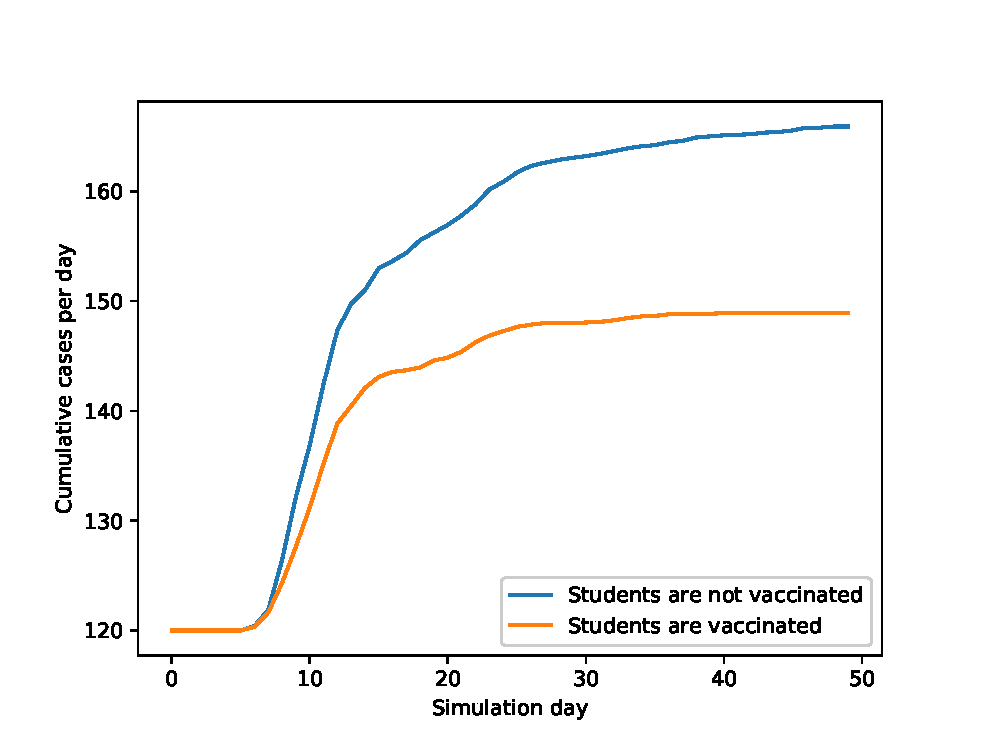
\includegraphics[width=\textwidth]{2_2_Vaccinating/vaccinating_cases_cum_20runs.eps}
		\caption{Plot showing the amount of infected people per day.} 	
	\end{subfigure}
	\begin{subfigure}[b]{0.7\linewidth}
		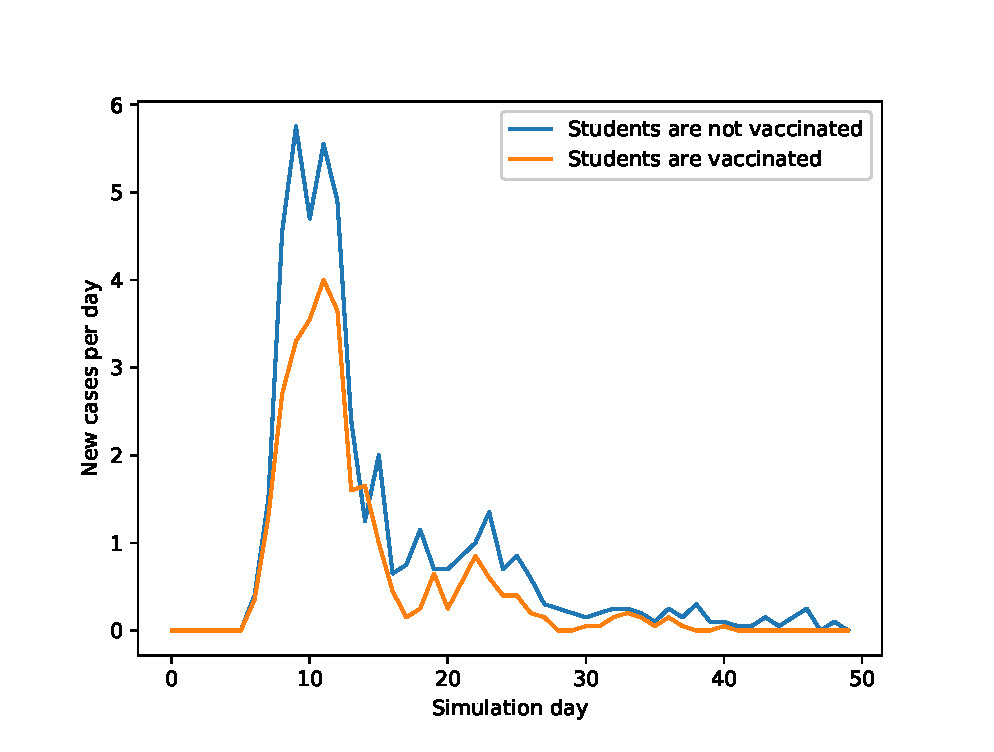
\includegraphics[width=\textwidth]{2_2_Vaccinating/vaccinating_cases_per_day_20runs.eps}
		\caption{Plot showing the amount of newly infected people per day.} 
	\end{subfigure}
	\caption{Plots showing the impact of vaccinating students. Averages from 20 simulations.}
	\label{VaccinePlot}
\end{figure}

\newpage

\subsection{Commuting to work}

\paragraph{} Another factor that is interesting to examine is the impact of commuting on disease spread. \\
In this simulation, we generate different populations, depending on different fractions of commuters. The expectation we have is that if more people commute to work, more people gets infected in the end. But when we run the simulation, we see that there isn't a difference between the fraction of commuters. We can also see that there is a peak between day 40 and 50. This peak doesn't change much when we increase the amount of commuters. If we increase the amount of days to 200, the peak is around 70-75, but still no difference between the fractions of commuters. 

\begin{figure}[h!]
	\centering
	\begin{subfigure}[b]{0.7\linewidth}
		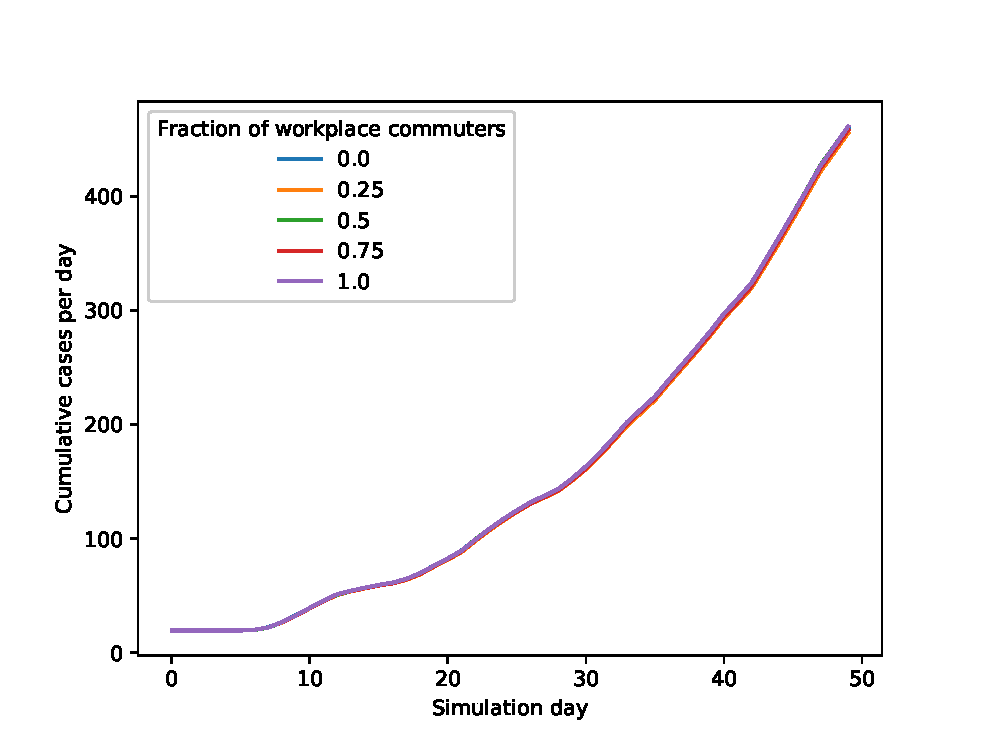
\includegraphics[width=\textwidth]{work_cum_1.eps}
		\caption{Cumulative cases per day} 
	\end{subfigure}
	\begin{subfigure}[b]{0.7\linewidth}
		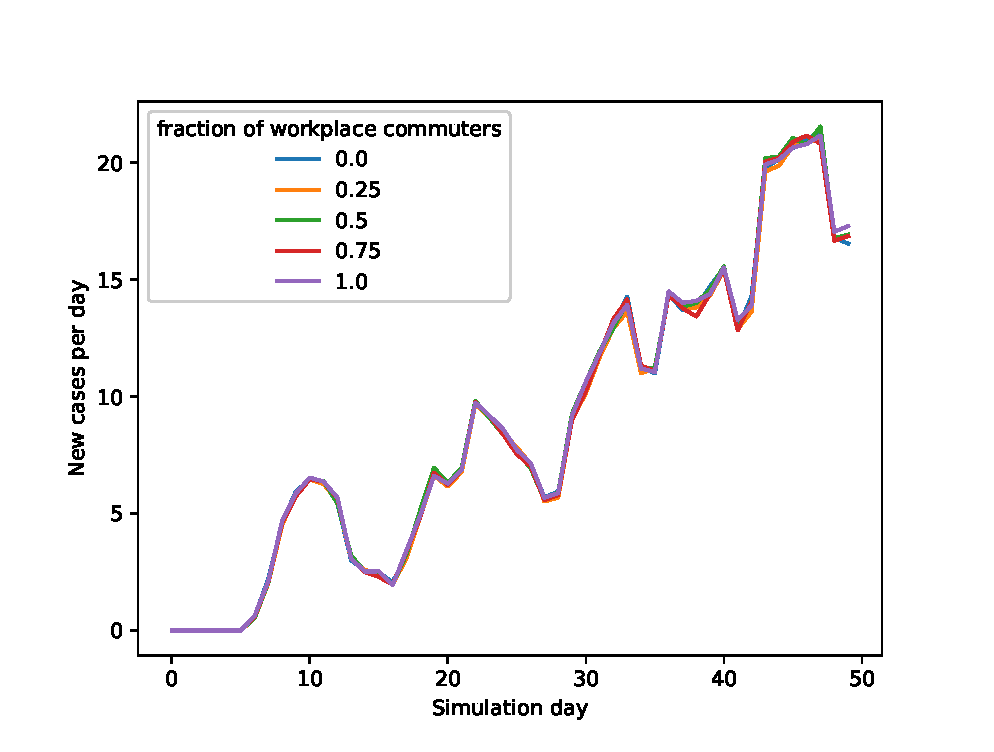
\includegraphics[width=\textwidth]{work_cases_per_day_1.eps}
		\caption{New cases per day.} 
	\end{subfigure}
	\caption{Plots showing the impact of Commuting to work on a population of size 10000. 1000 runs for each fraction. }
	\label{CommutingPlot1}
\end{figure}

\begin{figure}[h!]
	\centering
	\begin{subfigure}[b]{0.7\linewidth}
		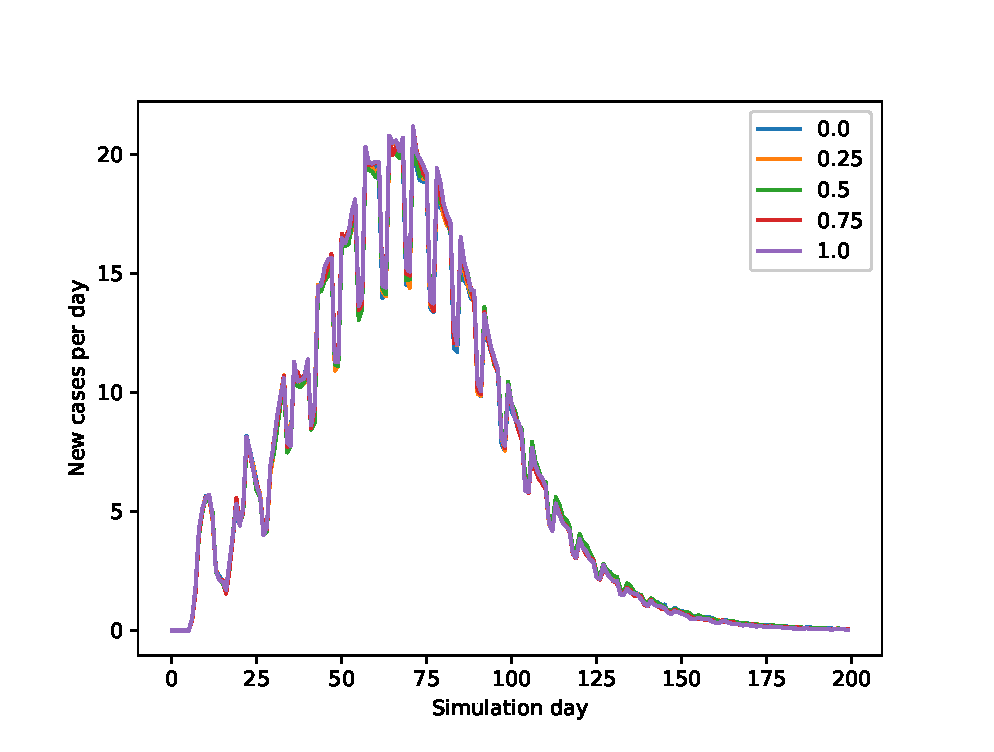
\includegraphics[width=\textwidth]{work_cases_per_day_3.eps}
		\caption{New cases per day.} 
	\end{subfigure}
	\caption{Plots showing the impact of Commuting to work on a population of size 10000. 1000 runs for each fraction. 200 days.}
	\label{CommutingPlot2}
\end{figure}

\newpage
When we increase the population size, we don't see many differences. 

\begin{figure}[h!]
	\centering
	\begin{subfigure}[b]{0.7\linewidth}
		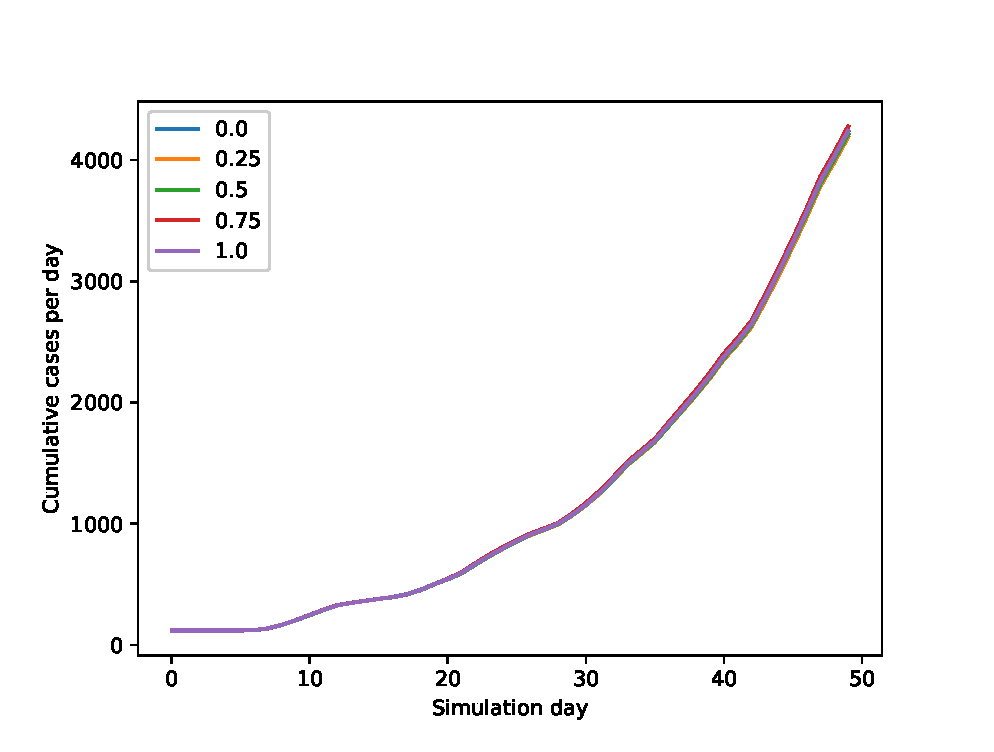
\includegraphics[width=\textwidth]{work_cum_2.eps}
		\caption{Cumulative cases per day} 
	\end{subfigure}
	\begin{subfigure}[b]{0.7\linewidth}
		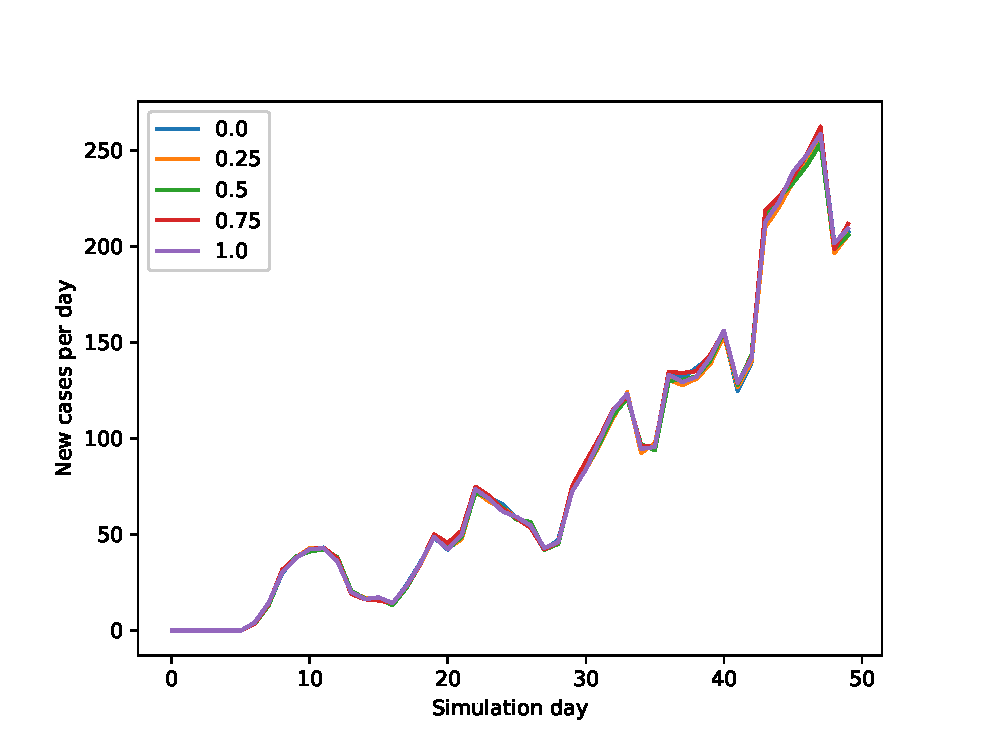
\includegraphics[width=\textwidth]{work_cases_per_day_2.eps}
		\caption{Plots showing the impact of Commuting to work on a population of size 600000. 100 runs for each fraction. } 
	\end{subfigure}
	\caption{Plots showing the impact of Commuting to work on a population of size 500000}
	\label{CommutingPlot3}
\end{figure}

\clearpage
\section{Performance profiling}

\paragraph{} Using GProf, a performance analysis tool, we will look at the impact of the following parameters:
\begin{itemize}
	\item Number of days
	\item Population size
	\item Immunity rate
	\item Seeding rate
	\item Contact log mode
\end{itemize}
on the performance of the Stride software.

\subsection{Number of days}

\paragraph{} By increasing the number of days to be simulated, the total execution time gets longer as well. This should be expected as more days means more times we simulate what goes on in a day.
\begin{figure}[h!]
\centering
	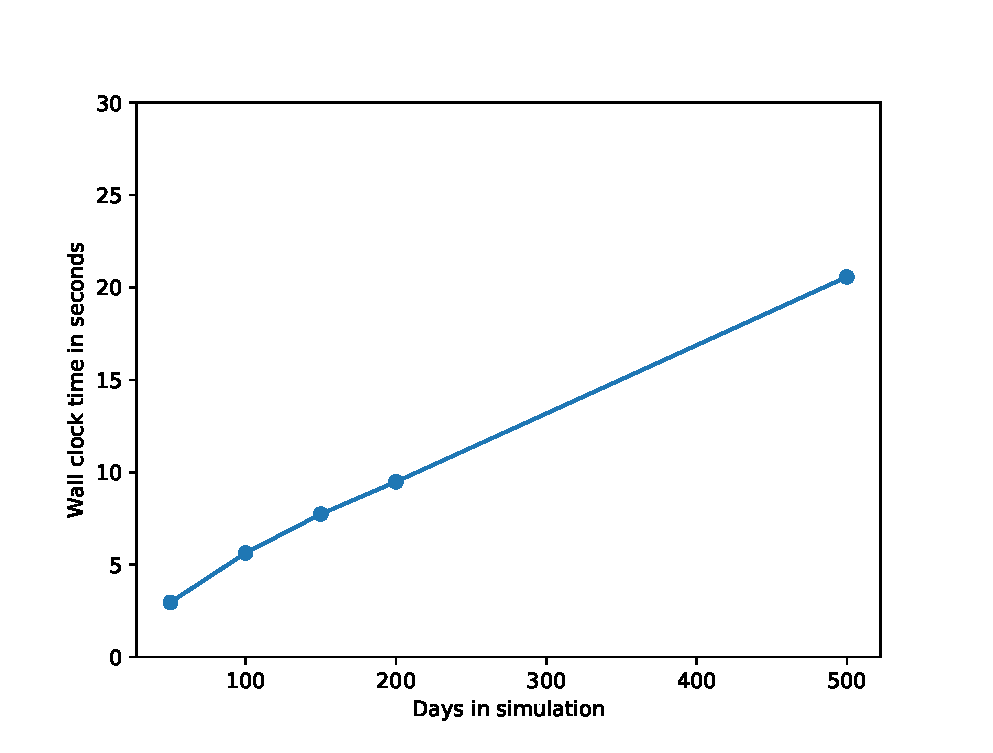
\includegraphics[width=0.8\textwidth]{3_Performance_Profiling/3_numdays.eps}
	\caption{Plot showing run time of simulations by varying the number of days.
			Average from 20 runs.} 
	\label{Gprof_numdays}
\end{figure}

\subsection{Population size}
\paragraph{} The time needed to generate a population scales linearly with the size of said population. And the same can be said about running the simulations. In figure \ref{Gprof_popsize} we can see that the simulation itself takes up more than half of the execution time.

\begin{figure}[h!]
	\centering
	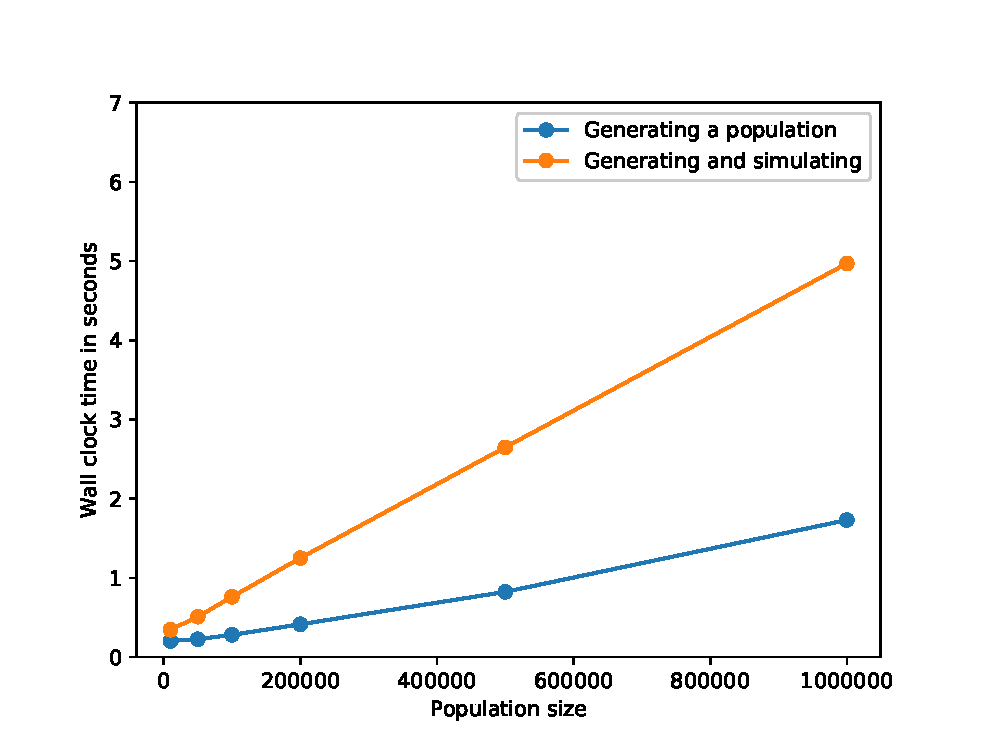
\includegraphics[width=\textwidth]{3_Performance_Profiling/3_popsize.eps}
	\caption{Plot showing run time when varying the size of the population.
			Average from 20 runs for each population size. Simulated over 50 days.}
	\label{Gprof_popsize}
\end{figure}

\subsection{Immunity rate}
\paragraph{} Varying the immunity rate does not seem to affect the total execution time.
In the case of generating a population this happens as for each person you need to determine whether they are immune to the disease, regardless of the immunity rate.

\begin{figure}[h!]
\centering
	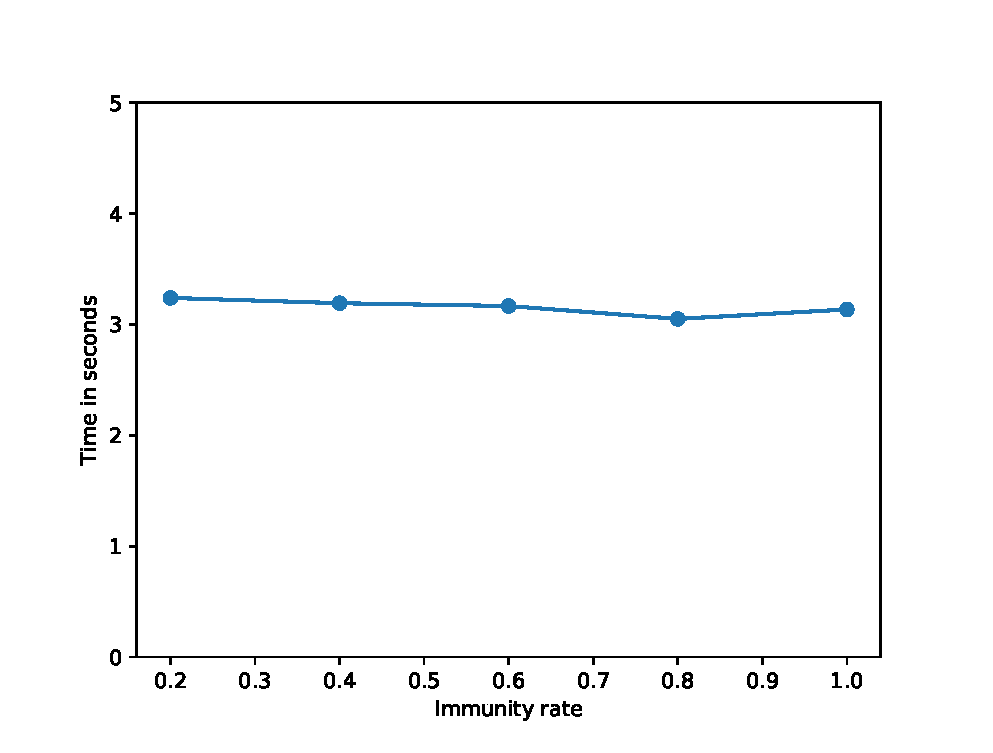
\includegraphics[width=0.8\textwidth]{3_Performance_Profiling/3_immunityrate.eps}
	\caption{Plot showing run time of simulations by varying the immunity rate.
			Average from 20 runs for each immunity rate. Simulated over 50 days.
	Averages of 20 runs.} 
	\label{Gprof_immunityrate}
\end{figure}

\subsection{Seeding rate}

\paragraph{} The seeding rate does not seem impact the time needed to generate the population. When you simulate however a larger seeding rate slightly increases the time of the execution. This happens as if a substantial amount of people is initially infected, more infections will happen in the subsequent timesteps.
We were unable to find results for seeding rates > 0.2 due to the limitations of the simulator.
\begin{figure}[h!]
\centering
	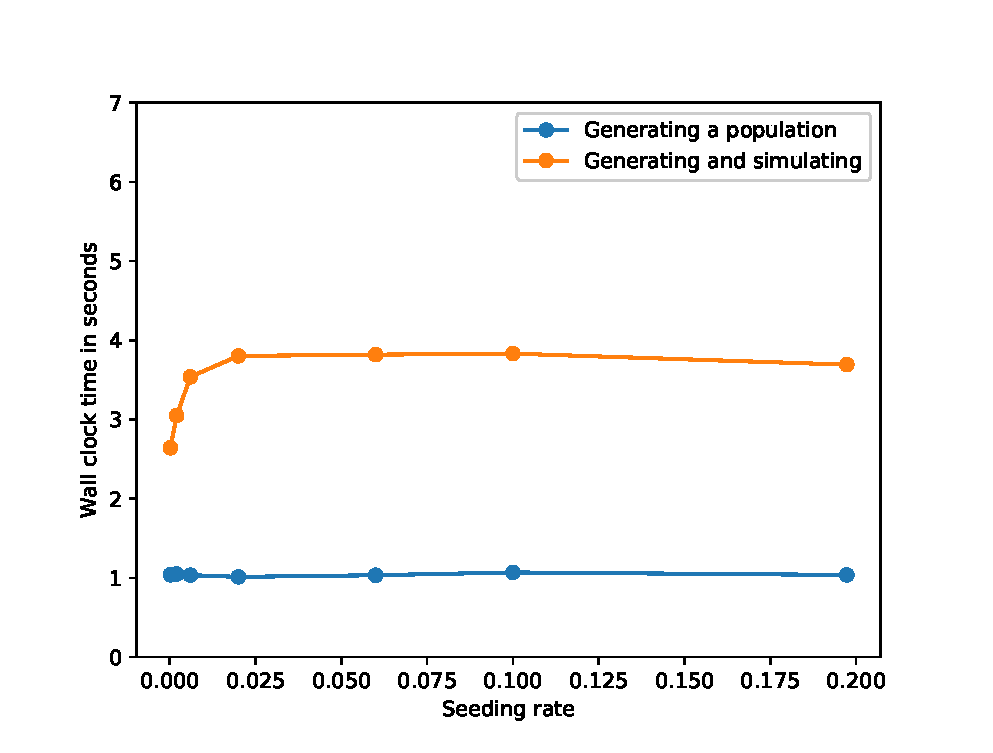
\includegraphics[width=0.8\textwidth]{3_Performance_Profiling/3_seedingrate.eps}
	\caption{Plot showing run time of simulations by varying the seeding rate.
	Averages from 20 runs for each seeding rate. Simulated over 50 days.} 
	\label{Gprof_seedingrate}
\end{figure}

\subsection{Contact log mode}

\paragraph{} The different contact logging modes are:
\begin{itemize}
	\item None
	\item Transmissions
	\item All
	\item Susceptibles
\end{itemize}

The mode of the contact log has a very large impact on the execution time
At day 50 in the simulation, only 20000 people out of 600000 where infected. When logging the susceptible people, you actually log almost 580000 people at each day which is very close to logging all people. This is very fast when the mode is set to Transmissions as you would only log once for each newly infected person. The logging modes 'All' and 'Susceptibles' use a less efficient algorithm, hence the big difference in run time between them and the modes 'Transmissions' and 'None'.

\begin{figure}[h!]
\centering
	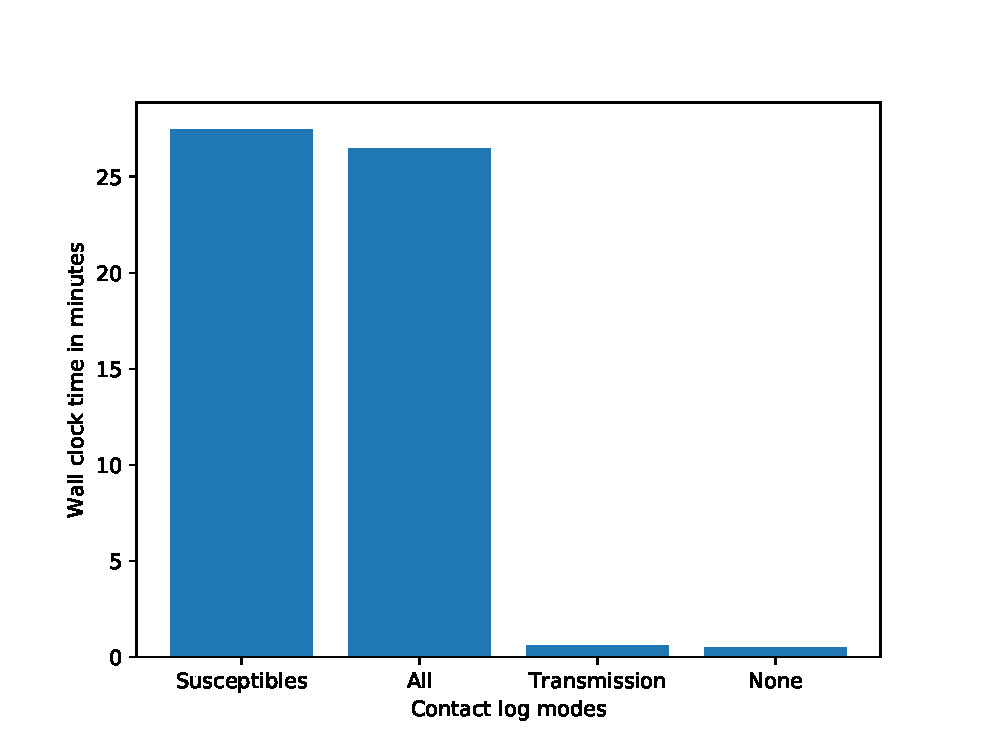
\includegraphics[width=0.8\textwidth]{3_Performance_Profiling/3_contactlogmode.eps}
	\caption{Plot showing run time of simulations using different logging methods.} 
	\label{Gprof_contactlogmode}
\end{figure}

\subsection{Impact on the code}
For the first 4 parameters
\begin{itemize}
	\item Number of days
	\item Population size
	\item Immunity rate
	\item Seeding rate
\end{itemize}
the actual sorting and analyzing of the population takes up most of the time.


\end{document}
